% ============================================================================
\section{RQ4 and robustness: what reaches the vendors, and how stable the measurements are}\label{sec:application}
% ============================================================================

\subsection{What reaches the vendors}\label{sec:app-url}

Every WPM event carries the page URL (Section~\ref{sec:bg-shopify}), so a choice changes which pixels start, not what a pixel that starts receives. In the Default load, 63.4\% (60.9--66.0\%) of the 10,676 sandboxed ad beacons on 769 stores carried the full landing URL with our canary token, and on 725 of 1,358 stores (53.4\%) at least one sandboxed beacon did (Fig.~\ref{fig:reach}c; by arm: Supplementary Fig.~\ref*{S:fig:s9}a); the share was 95.8\% for TikTok's sandboxed beacons and 87.1\% for Pinterest's.

\begin{widefig}
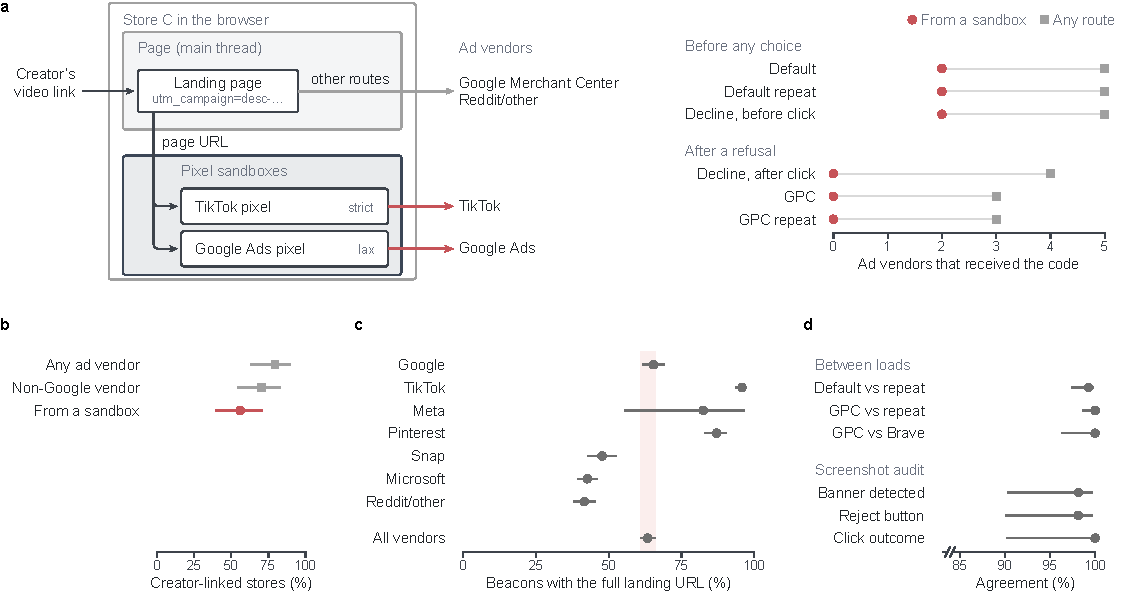
\includegraphics{fig6.pdf}
% GENERATED by paper/integrate_figures_v2.py from figures/v7/fig6/caption_fig6.tex (v2 figure caption, rendered by the figure script).
% Do not edit: change the figure script and re-run build.sh.
\caption{\textbf{Ad vendors receive the landing URL, including a creator's per-video code, and the measurements behind this repeat across loads and agree with a screenshot audit.} (a)~Store~C, a creator-linked store, loaded from a creator's video link whose uniform resource locator (URL) carries a per-video code (`utm\_campaign=desc-\ldots', the video's identifier elided here and in the drawing). Left: the code's path, on the regions of Fig.~\ref{fig:situating}a (outline: the browser; light grey ground: the page's main thread; darker grey ground: the pixel sandboxes). The landing page hands its URL to the pixels that Shopify runs in sandboxes isolated from the page, TikTok's pixel in a web worker (strict runtime) and Google Ads' pixel in a sandboxed iframe (lax runtime), and they send the code to the ad vendors outside the browser (brick arrows); scripts outside the sandboxes can send it as well (grey arrow: other routes). The ad vendors that received the code in the Default load are named at the heads of the paths that reached them. Right: one row per load of Store~C, in two groups. Before any choice: Default, its repeat, and a Decline load before the click on the banner's reject button; after a refusal: the same Decline load after the click (the rest of that page and the fresh page after the reload), a Global Privacy Control (GPC) load and its repeat (GPC refuses from the start). Brick circles: ad vendors that received the code from a sandbox; grey squares: ad vendors that received it by any route; a light line joins the two counts of a load. In each of the three loads before any choice the code reached 5 ad vendors (Google Ads, Google Merchant Center, TikTok and vendors in the Reddit/other group), 2 of them, TikTok and Google Ads, from a sandbox; TikTok's sandboxed pixel sent it in 4 requests per load. After the Decline click it still reached 4 vendors and under GPC 3, 0 of them from a sandbox, with 0 requests from TikTok's sandbox. (b)~All 34 creator-linked stores, Default load: share of stores on which the creator's code reached any ad vendor, 79.4\% (27 of 34), a vendor other than Google, 70.6\% (24 of 34), and an ad vendor from a sandbox, 55.9\% (19 of 34); Wilson 95\% confidence intervals (CIs) 63.2--89.7\%, 53.8--83.2\% and 39.5--71.1\% (horizontal lines). Marks as in (a): grey squares, by any route; brick circle, from a sandbox. (c)~Sandboxed ad beacons in the Default load that carried the full landing URL with our test code, by vendor group in a fixed order (dark grey circles; lines: Korn--Graubard 95\% CIs clustered by store): Google 65.4\% (2,689 of 4,112 beacons); TikTok 95.8\% (1,387 of 1,448); Meta 82.5\% (33 of 40); Pinterest 87.1\% (978 of 1,123); Snap 47.7\% (199 of 417); Microsoft 42.6\% (376 of 882); Reddit/other 41.7\% (1,106 of 2,654). Groups with fewer than 10 stores would be omitted; the smallest shown, Meta, has 40 beacons on 18 stores. Bottom row, set apart: all vendors, 63.4\% of 10,676 beacons on 769 stores (95\% CI 60.9--66.0\%, resampling stores); this interval is carried up through the vendor rows as a pale brick band (as the main estimates in Fig.~S5; these beacons left a sandbox before any choice), so each vendor group reads against all vendors. (d)~Robustness (dark grey circles; lines: Wilson 95\% CIs), in two named groups. The agreement axis is truncated (it does not start at zero; the break mark at its left end shows the cut); every interval ends right of the break. Between loads: agreement between two loads of the same store on whether a sandboxed ad pixel sent a request, for the validation loads, that is, repeats of Default and GPC (273 stores) and Brave's native GPC (98 stores): Default vs repeat 99.3\% (271 of 273; Cohen's $\kappa$ 0.985, 95\% CI 0.961--1.000), GPC vs repeat 100.0\% (273 of 273), emulated GPC vs Brave 100.0\% (98 of 98). Screenshot audit: the crawler's labels against saved screenshots: banner detections confirmed 98.1\% (53 of 54), first-layer reject button 98.1\% (52 of 53), click outcome 100.0\% (35 of 35). The audit labels have not yet been checked by an independent human rater. Details: Fig.~S4. In (a) and (b), brick marks the code leaving from a Shopify sandbox (consent lost) and grey marks any route. By arm, with the refusal signals that vendors receive in ad requests: Fig.~S9.
Panel~(a), left: Drawn by figure-generation scripts written with AI assistance (Section~\ref{sec:method-ai}).}
\label{fig:reach}

\end{widefig}

Some vendors register a refusal in their own layer (Supplementary Fig.~\ref*{S:fig:s9}b--c). Of Google requests of any origin, 35.6\% on the next page after a Decline and 49.3\% under GPC carried a refusal signal, as did 19.6\% and 9.6\% of Microsoft's, but almost none of the other vendors' (0.7\% under GPC). The sandboxed residuals are not explained by such signals: every remaining sandboxed request carried one on only 9 of the 53 stores with a fresh-page residual after Decline and on 18 of the 279 with a residual under GPC. Signals were read from request URLs only, so these shares are lower bounds.

\subsection{Creator links: the motivating case}\label{sec:app-creator}

On the 34 creator-linked stores, a purposive sample, the creator's code reached an ad vendor in the Default load on 27 stores, a vendor other than Google on 24, and did so from a Shopify sandbox on 19 (Fig.~\ref{fig:reach}b). Codes that name a single video reached a vendor other than Google on 3 of the 6 landing pages that carried one, so the per-video flow is not unique to \storeC, our case study (Fig.~\ref{fig:reach}a; all five loads: Supplementary Fig.~\ref*{S:fig:s9}d). On \storeC, TikTok's STRICT pixel sent the per-video code in 4 requests in each of the Default, repeat and pre-click Decline loads, and under GPC TikTok sent nothing (further detail and an edge-cache effect: Supplementary \ref*{S:sec:s-gate} and~\ref*{S:sec:s-extended}).

\subsection{Robustness and validity}\label{sec:app-validation}

\emph{Stability.} Whether a sandboxed ad request fired was stable across repeat loads (Fig.~\ref{fig:reach}d; Supplementary Fig.~\ref*{S:fig:s4}d): Default versus repeat Default agreed on 271 of 273 stores (Cohen's $\kappa=0.985$, 95\% CI 0.961--1.000) and GPC versus repeat GPC on 273 of 273. The Decline arm had no repeat load, and the timing flag repeated only moderately (Section~\ref{sec:res-prechoice}).

\emph{Emulated versus native GPC.} Brave's native GPC and our emulation agreed on whether a sandboxed ad request fired on 98 of 98 stores and 686 of 686 store--vendor pairs. Pixel code in STRICT workers read \code{navigator.globalPrivacyControl} as undefined in all 4,720 workers under emulation and 382 under Brave \citep{shopify_aboutpixels}, so on Shopify GPC acts only through Shopify's consent state and the request header, although the standard exposes it to workers \citep{w3c_gpc}.

\emph{What the pages saw of our crawler.} Every page could tell that our browser was automated: \code{navigator.webdriver} was true and the user agent contained ``HeadlessChrome'' in all 4,840 usable loads with a page probe. In the saved code of the consent tools, Pandectes' version 5 has a merchant setting, off by default according to the vendor, that for such browsers hides the banner and grants consent, which it passes to Shopify as ordinary implied consent; its signature appeared in the Default and GPC loads of 5 stores, while 31 version-5 stores configured as opt-in for California showed their banner and wrote nothing (other tools: Supplementary Table~\ref*{S:tab:s-detection}). A setting that grants consent to automated browsers makes pixels fire where a person would first see an opt-in banner, which is why the blocked-on-paper primary excludes every store whose CMP wrote ``yes''.

\emph{Sensitivity, audits and recall.} All 20 robustness variants of the three headline rates gave intervals that overlapped the main estimates (Supplementary Fig.~\ref*{S:fig:s5}), weak evidence because most variants are near-subsets of the main sample; a comparison of the six- and ten-browser crawl segments was underpowered (Supplementary \ref*{S:sec:s-sens}). In the screenshot audit of 54 seeded Decline loads, 53 detected banners were real and the reject finder agreed with the screenshots on 52 of 53, and the banner detector's recall on re-check screenshots was about 91\% (73--96\%) (Supplementary \ref*{S:sec:s-audit}). These labels are not yet an independent validation (Section~\ref{sec:method-ai}).

\subsection{Projection to the DNS frame}\label{sec:app-projection}

Weighted to the about 2,444 eligible storefronts in the DNS frame (Table~\ref{tab:projection}), about 383 stores (15.7\%, 13.5--17.9\%) show a consent banner while sending sandboxed ad requests before any choice, and with GPC switched on about 512 (20.9\%, 18.5--23.4\%) keep sending sandboxed ad requests, while at most about 7 would send them from a pixel that declares sale of data (an approximate, unweighted bound). The projections hold for the DNS frame only, whose recall is about 83\% (Section~\ref{sec:method-sample}), and no interval includes this coverage error (Supplementary \ref*{S:sec:s-extended}).

\begin{table}[!tbp]
\centering
\caption{Projection to the about 2,444 DNS-flagged storefronts in the Tranco top 200,000 (Section~\ref{sec:method-sample}), stratified by rank bucket with design weights; intervals are design-based and include the uncertainty of the frame size.}
\label{tab:projection}
\small
\tabinput{tables/table_projection.tex}%
\end{table}
